\chapter{Introduction}

\section{Motivation}
% are these words too informal?
Fluids can be seen everywhere. The smoke rising from the chimney and spreading in the wind, the milk in a cup mixing with the coffee, the calm flow of a river with tiny ripples under the rain, and the violent waves of the ocean shooting up and splashing down. Many of these phenomena have stunning visual effects, and quite often, realistic images of these fluids need to be computationally generated for purposes such as cinematics and video games. 


Due to the mathematical complexity underlying the motion of fluids, accurate numerical simulations often require a vast amount of computation time. However, real-time computer graphics applications, such as video games, usually require the simulation to be computed in approximately the same amount of time as the physical process it represents. Moreover, in these applications, it is often required that the results of the simulation (i.e, the shape and motion of the fluid) are realistically rendered and displayed to the user. This project studies how these demands can be met on modern machines: by utilizing the parallel computing abilities of GPUs.




\section{Related Work}



The study of the behavior of fluids dates back to 18th century, when Leonhard Euler proposed a set of partial differential equations (PDEs), known as \textit{\ref{eqn:Euler Equations}}, that govern the behavior of an idealized incompressible and inviscid fluid. In the 19th century, these equations were extended by Claude-Louis Navier and George Gabriel Stokes into the famous \textit{\ref{eqn:Navier-Stokes Equations}}, which describe a much broader class of fluids that occur in the real world. These equations are explained in greater detail in chapter \ref{chapter physics}, and they are exactly what most fluid simulation software, including the one implemented in this project, are trying to solve. 

Somewhat unfortunately, the Euler and Navier-Stokes equations have extremely difficult mathematical properties, and general analytical solutions are yet to be found even today. As a result, fluid simulation software resort to numerical methods to approximate solutions. In computer graphics applications, there are two prominent families of numerical methods for solving the fluid equations: the grid-based methods and the particle-based methods. Each approach comes with its own benefits and drawbacks, but could both be implemented efficiently on GPUs to achieve real-time simulation.

The grid-based methods rely on spatial discretizations of the scalar and vector fields that represent the fluids. The most widely used discretization method, the \textbf{MAC} (Marker and Cell) \textbf{grid}, was proposed by Harlow and Welch\cite{harlow1965numerical} in 1965. Known for its high accuracy, this discretization scheme is the basis of most grid-based fluid simulation algorithms. 

A significantly important step during a grid-based simulation is to move all the physical quantities stored in the grid (e.g. concentration) according to the velocity field. This step, known as \textit{advection}, essentially determines how the shape of the fluid evolves over time. Thus, it is key to a high-fidelity simulation. A few popular advection algorithms include \textbf{MacCormack}\cite{selle2008unconditionally} and \textbf{BFECC}\cite{kim2005flowfixer}, both of which have efficient GPU implementations\cite{chentanez2011real}\cite{xu2011interactive}. This project chooses to implement the advection algorithm known as \textbf{FLIP} (Fluid Implicit Particle)\cite{zhu2005animating}, developed by Zhu and Bridson. This algorithm, interestingly enough, makes uses of particles to move quantities within the MAC grid. FLIP has various advantages over the purely grid-based algorithms, and is likely the most widely used advection method nowadays. The name FLIP consequently became a commonly used abbreviation for the full grid-based simulation with FLIP advection.

As an addition to the traditional single-phase fluid simulation, Kang\cite{kang2010hybrid} showed how to extend the grid-based algorithms to capture the diffusion between multiple miscible fluid phases (e.g. red ink spreading in transparent water). This project implements a modified version of the proposed algorithm, where FLIP, rather than BFECC, is used to advect the concentration of different fluid phases.



Apart from grid-based simulations, there is also a family of particle-based fluid simulation algorithms called \textbf{SPH} (Smoothed Particle Hydrodynamics), which does not rely on a grid. Originally developed for astronomical simulations by Lucy\cite{lucy1977numerical} and Monaghan\cite{monaghan1992smoothed} in 1977, SPH was introduced to computer graphics in 2003 by Müller\cite{muller2003particle}. The SPH method represents the fluid by a moving cloud of particles, which carry the physical quantities of the fluid with them. Two extensions of the SPH algorithm, namely PCISPH\cite{solenthaler2009predictive} and PBF\cite{macklin2013position}, was studied and implemented in the early phases of this project. However, it was found that they could not match the performance and accuracy of the FLIP algorithm. It was therefore decided that this project will focus mainly on FLIP.



On the rendering side, this project follows the proposal by Zhu and Bridson\cite{zhu2005animating}, who showed how a particle representation of a fluid could be used to compute a signed distance field, which represents the distance to the fluid surface of each point in the 3D space. An algorithm known as Marching Cubes, invented by Wyvill\cite{wyvill1986soft} and Lorensen\cite{lorensen1987marching}, can then use this field to reconstruct the fluid's surface as a triangle mesh representation, which is suitable for rendering. Alternatively, screen-space algorithms\cite{van2009screen} can be used, which do not generate a triangle mesh but directly uses the particles for rendering.



\section{Project Outline}


This project focuses on studying the FLIP fluid simulation algorithm and its GPU parallelization. The project extends the original FLIP, giving it the ability to simulate multiple fluids of different densities and colours, while capturing the diffusion phenomenon between them. In order to create an efficient GPU implementation of the algorithm, the project identifies parts of it that are not straightforwardly parallelizable, and overcomes these difficulties by investigating and implementing certain auxiliary parallel subroutines. Various memory access optimizations are also performed, so that the resulting implementation fully exploits the GPU's computation power and is fast enough to be used in real-time applications.

To visualize the simulations, the project implements a fast surface reconstruction algorithm, which transforms a particle cloud representation of fluids into a renderable triangle mesh. A real-time renderer is implemented to render the mesh while capturing all the reflection and refraction phenomena that occur in the real world. Furthermore, the renderer incorporates a novel algorithm that computes the different levels of attenuation of light caused by fluids of different colours, thereby also realistically rendering the liquid diffusion effects. 

Integrating the simulation and rendering, the project creates a fully-featured program, which allows the user to easily set up a fluid simulation and obtain a rendered animation. The user can configure the shapes and sizes of the fluid before the simulation starts, as well as the initial colour and transparency of each fluid volume. The program can then carry out the simulation and render realistic results to the user in real time. 

The software is developed for GPUs manufactured by the NVIDIA Cooperation, and utilizes NVIDIA's CUDA programming model. The OpenGL graphics API is used to interact with the GPU to render the fluid. The majority of the software consists of C++ code written for the CPU side of the program, and CUDA code for the GPU side. Additionally, a comparatively smaller amount of GLSL code is written specifically for rendering. With a total of over 13 thousand lines, the complete source code of the software can be found at \url{https://github.com/AmesingFlank/Aquarius}, along with some additional information and screenshots.

\begin{figure}[H]
    \centering
        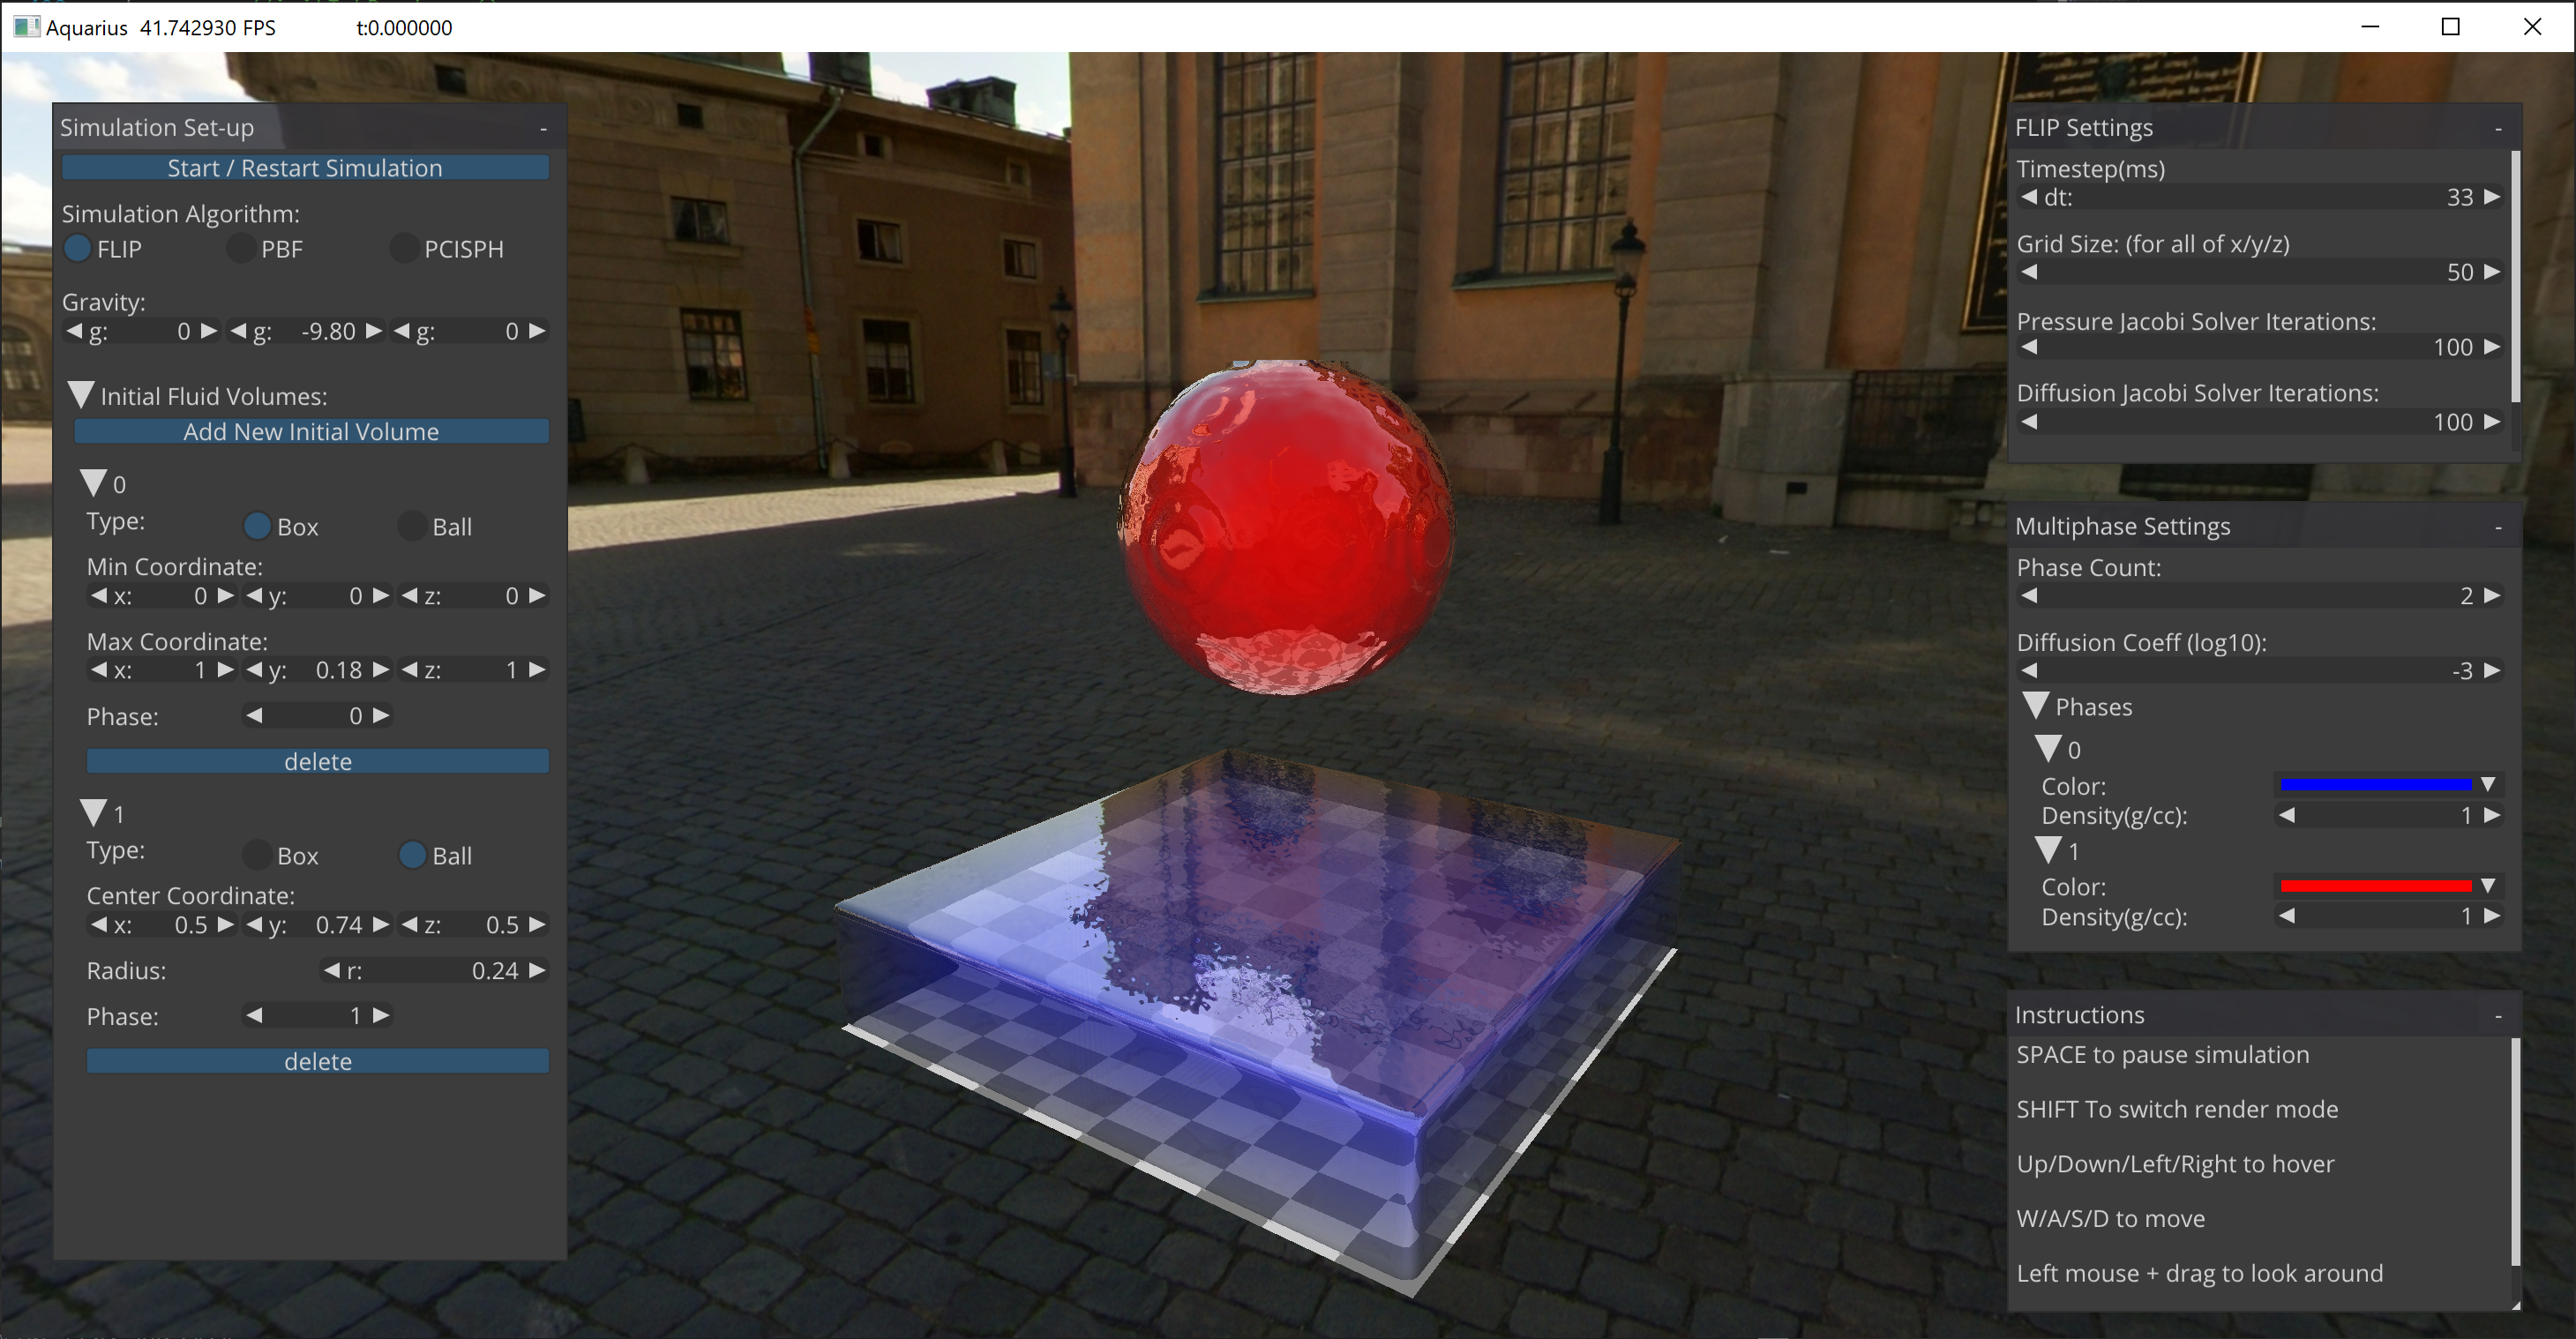
\includegraphics[width=15.2cm]{UI}
    \caption{The full user interface of the software}
    \label{figure UI demo}
\end{figure}